\documentclass[11pt,]{article}
\usepackage{lmodern}
\usepackage{amssymb,amsmath}
\usepackage{ifxetex,ifluatex}
\usepackage{fixltx2e} % provides \textsubscript
\ifnum 0\ifxetex 1\fi\ifluatex 1\fi=0 % if pdftex
  \usepackage[T1]{fontenc}
  \usepackage[utf8]{inputenc}
\else % if luatex or xelatex
  \ifxetex
    \usepackage{mathspec}
  \else
    \usepackage{fontspec}
  \fi
  \defaultfontfeatures{Ligatures=TeX,Scale=MatchLowercase}
  \newcommand{\euro}{€}
\fi
% use upquote if available, for straight quotes in verbatim environments
\IfFileExists{upquote.sty}{\usepackage{upquote}}{}
% use microtype if available
\IfFileExists{microtype.sty}{%
\usepackage{microtype}
\UseMicrotypeSet[protrusion]{basicmath} % disable protrusion for tt fonts
}{}
\usepackage[margin=1in]{geometry}
\usepackage{hyperref}
\PassOptionsToPackage{usenames,dvipsnames}{color} % color is loaded by hyperref
\hypersetup{unicode=true,
            pdftitle={Are environmental and geographic variables effective surrogates for genetic variation in conservation planning?},
            pdfborder={0 0 0},
            breaklinks=true}
\urlstyle{same}  % don't use monospace font for urls
\usepackage{graphicx,grffile}
\makeatletter
\def\maxwidth{\ifdim\Gin@nat@width>\linewidth\linewidth\else\Gin@nat@width\fi}
\def\maxheight{\ifdim\Gin@nat@height>\textheight\textheight\else\Gin@nat@height\fi}
\makeatother
% Scale images if necessary, so that they will not overflow the page
% margins by default, and it is still possible to overwrite the defaults
% using explicit options in \includegraphics[width, height, ...]{}
\setkeys{Gin}{width=\maxwidth,height=\maxheight,keepaspectratio}
\setlength{\parindent}{0pt}
\setlength{\parskip}{6pt plus 2pt minus 1pt}
\setlength{\emergencystretch}{3em}  % prevent overfull lines
\providecommand{\tightlist}{%
  \setlength{\itemsep}{0pt}\setlength{\parskip}{0pt}}
\setcounter{secnumdepth}{0}

%%% Use protect on footnotes to avoid problems with footnotes in titles
\let\rmarkdownfootnote\footnote%
\def\footnote{\protect\rmarkdownfootnote}

%%% Change title format to be more compact
\usepackage{titling}

% Create subtitle command for use in maketitle
\newcommand{\subtitle}[1]{
  \posttitle{
    \begin{center}\large#1\end{center}
    }
}

\setlength{\droptitle}{-2em}
  \title{Are environmental and geographic variables effective surrogates for
genetic variation in conservation planning?}
  \pretitle{\vspace{\droptitle}\centering\huge}
  \posttitle{\par}
  \author{Jeffrey O. Hanson\(^1\), Jonathan R. Rhodes\(^2\), Cynthia
Riginos\(^1\), Hugh P. Possingham\(^1\), Richard A. Fuller\(^1\)\\
\(^1\)School of Biological Sciences, The University of Queensland,
Brisbane, QLD, Australia\\
\(^2\)School of Geography, Planning and Environmental Management, The
University of Queensland, Brisbane, QLD, Australia\\
Correspondance should be addressed to
\href{mailto:jeffrey.hanson@uqconnect.edu.au}{\nolinkurl{jeffrey.hanson@uqconnect.edu.au}}}
  \preauthor{\centering\large\emph}
  \postauthor{\par}
  \predate{\centering\large\emph}
  \postdate{\par}
  \date{07 May 2016}


% load packages
\usepackage{amsmath,amsfonts,float,makecell,titletoc,tocloft,titlesec,natbib,pdfpages,lineno,booktabs}
\usepackage[T1]{fontenc}
\usepackage{lmodern}
\usepackage[utf8]{inputenc}
\usepackage[doublespacing]{setspace}

% format captions
\usepackage[labelfont={small,bf}, labelsep=space, font={small}]{caption}

% format headings
\titleformat{\subsection}
{\normalfont\Large\bfseries}{\thesubsection}{1em}{}
\titleformat{\subsubsection}
{\normalfont\large\bfseries}{\thesubsubsection}{1em}{}
\titleformat{\paragraph}
{\normalfont\normalsize\bfseries}{\theparagraph}{1em}{}
\titleformat{\subparagraph}
{\normalfont\normalsize\itshape}{\thesubparagraph}{1em}{}

\titlespacing\paragraph{0pt}{12pt plus 4pt minus 2pt}{+0pt plus 2pt minus 2pt}
\titlespacing{\subparagraph}{0pt}{6pt plus 4pt minus 2pt}{+0pt plus 2pt minus 2pt}

% format toc
\renewcommand\cftsubsecfont{\normalfont\normalsize\bfseries}
% \renewcommand\cftsubsubsecfont{\normalfont\normalsize\bfseries}
% \renewcommand\cftparafont{\normalfont\normalsize\bfseries}
% \renewcommand\cftsubparafont{\normalfont\normalsize\itshape}

% make figures static
\let\origfigure\figure
\let\endorigfigure\endfigure
\renewenvironment{figure}[1][2] {
	\expandafter\origfigure\expandafter[H]
} {
	\endorigfigure
}

% define struts for tables
\newcommand\T{\rule{0pt}{2.6ex}} % top strut
\newcommand\B{\rule[-1.2ex]{0pt}{0pt}} % bottom strut

% define command to put new lines in table cells
%\newcommand{\specialcell}[2][c]{%
%  \begin{tabular}[#1]{@{}c@{}}#2\end{tabular}}

% Redefines (sub)paragraphs to behave more like sections
\ifx\paragraph\undefined\else
\let\oldparagraph\paragraph
\renewcommand{\paragraph}[1]{\oldparagraph{#1}\mbox{}}
\fi
\ifx\subparagraph\undefined\else
\let\oldsubparagraph\subparagraph
\renewcommand{\subparagraph}[1]{\oldsubparagraph{#1}\mbox{}}
\fi

\begin{document}
\maketitle
\begin{abstract}
Insert abstract here.
\end{abstract}

Short running title: Genetic surrogates in conservation \newline
Word count: XXXXX \newline
Number of references: XXXX \newline
Number of figures: XXXX \newline
Number of tables: XXXX \newline
Number of text boxes: XXXX \newline
\newpage

\subsection{Introduction}\label{introduction}

Protected areas spearhead conservation efforts (Sanderson \emph{et al.}
2015). These places buffer species from anthropogenic impacts and
provide places for species to persist. However, the resources available
for conservation are limited. Thus protected areas need to be sited in
places that achieve conservation goals for minimal cost. To ensure that
protected areas are cost-effective, plans for protected areas
(prioritizations) are often generated using decision support tools to
identify near-optimal solutions. Additionally, because reserves cannot
preserve the entire range for a given species, the plans for multiple
reserves are often designed simultaneously to ensure that the network of
protected areas can facilitate biological processes (eg. gene flow
between populations, seasonal migration). For instance, \texttt{Marxan}
(Ball \emph{et al.} 2009) uses amount-based targets to identify
protected area networks that preserve a suitable amount of habitat for
each species (eg. 100 km \(^2\) of land occupied by the species needs to
be secured in a reserve) and weights to penalize fragmented solutions.
However, conservation planning exercises typically assume that all
individuals in the same species are equivalent.

Intra-specific genetic variation is an important for long-term species
persistence. As a consequence, there has been increasing interest in
designing prioritizations that preserve and cultivate this variation
(Moritz 1999; Crandall \emph{et al.} 2000; Hendry \emph{et al.} 2010).
Although the strength of natural selection is a continuous force;
broadly speaking, genetic variation can be classified as either adaptive
or neutral (reviewed in Schoville \emph{et al.} 2012). Adaptive genetic
variation is associated with loci that (significantly) affect fitness.
Typically, such ``adaptive'' loci are detected due to anomalous patterns
among individuals (eg. Foll \& Gaggiotti 2008; Duforet-Frebourg \emph{et
al.} 2014; Schoville \emph{et al.} 2012; Whitlock 2015; but see Rellstab
\emph{et al.} 2015 for alternative methods). By preserving existing
patterns of adaptive variation, protected areas can ensure that
populations with particularly beneficial adaptations are not lost
(Crandall \emph{et al.} 2000). In contrast, neutral genetic variation is
associated with loci that do not (significantly) affect fitness. Neutral
variation often reflects the evolutionary history of different
populations. By preserving existing patterns of neutral variation,
protected areas can secure different genetic lineages and avoid the
adverse effects of low genetic diversity (eg. inbreeding depression;
Moritz 1999). Thus protected area networks should preserve both adaptive
and neutral patterns of genetic variation for species of conservation
interest (Moritz 1999; Crandall \emph{et al.} 2000). Despite this,
genetic data are not often used to inform prioritizations because they
require considerable investment to obtain and analyze (Hendry \emph{et
al.} 2010; but see Moritz 1994 for developments on using genetic data in
conservation planning). Thus prioritizations may fail to capture
species' intra-specific genetic variation, and ultimately fail to
deliver long-term conservation outcomes.

Recently, conservation scientists have been investigating surrogates to
generate prioritizations that adequately preserve genetic variation--but
without actually needing to utilize genetic data to do this. Since
adaptive genetic variation is ultimately driven by extrinsic selection
pressures, environmental variables have been used to guide reserve
selection (eg. environmental conditions; Pyke \& Fischer 2005; Carvalho
\emph{et al.} 2011). By preserving a more representative sampled of
environmental conditions across the species' ranges, they aimed to
generate prioritizations that preserved more adaptive variation.
However, the effectiveness of this approach remains unverified. On the
other hand, neutral genetic variation arises from a reduction in gene
flow between individuals. Surrogates for neutral variation have been
based on variables that predict the level of connectivity between
planning units. For instance, the isolation by distance theory (IBD;
Wright 1943) predicts that populations further apart will have less
connectivity, exchange less genetic material, and in turn have less
genetic variation in common. Based on this theory, geographic
distance-based surrogates have been found to improve prioritizations in
an island network (Ponce-Reyes \emph{et al.} 2014). However this remains
untested in spatially contiguous systems where connectivity is
complicated by additional factors (eg. terrain; eg. Peterman \emph{et
al.} 2014a)--the very systems commonly featured in real-world
conservation planning exercises (eg. Cowling \emph{et al.} 2003). Before
conservation planners can reliably use surrogates for genetic data in
conservation planning, the effectiveness of these surrogates needs to be
verified. Otherwise, conservation planners may waste precious resources
on protecting places that provide little benefit to biodiversity.

Here we investigate the effectiveness of environmental and geographic
surrogates for adaptive and neutral genetic variation in the context of
conservation planning. First, we aim to verify if environmental and
geographic variables correlate with broad-scale patterns in adaptive and
neutral variation (respectively). Although these variables may correlate
with genetic variation, they may not be effective surrogates if the
level of correlation is not high enough or due to spatial
auto-correlative effects. Second, we aim to verify that environmental
and geographic variables are effective surrogates for adaptive and
neutral variation (respectively). We expect that prioritizations
generated using surrogate-based targets will secure more genetic
variation than prioritizations generated using only amount-based targets
with the same number of planning units. Third, we aim to determine if
the addition of surrogate-based targets to conservation planning
exercises can result in more effective prioritizations. We expect that
prioritizations generated using amount- and surrogate-based targets will
sufficiently preserve the genetic variation of more species than those
generated using only amount-based targets. If these surrogates can
improve the intra-specific genetic variation captured in a
prioritization, then conservation planners may use these surrogates when
genetic data is not available, and in turn deliver more effective
protected areas.

\subsection{Methods}\label{methods}

\subsubsection{Study system}\label{study-system}

We used species distribution and genomic data collected by the
IntraBioDiv project in the European Alps (Meirmans \emph{et al.} 2011;
see Gugerli \emph{et al.} 2008 for further explanation of data
collection methods). This data set contains information for 27 alpine
plant species (Figure 1a). It was collected using a 20' longitude by 21'
latitude grid (approx. 22.3 km \(\times\) 25 km; Figure S1). Project
members visited every second grid cell, and if a species was detected in
a cell, samples were collected from three individuals. They genotyped
samples using amplified fragment length polymorphisms (AFLP; Vos
\emph{et al.} 1995), and constructed matrices denoting the
presence/absence of polymorphisms at loci for each species (mean 132
\(\pm\) 55.6 SD markers genotyped per species; see Table 1 in Alvarez
\emph{et al.} (2009) for the number markers for each species). Although
AFLPs are not ideal as genomic representatives (cf.~single nucleotide
polymorphisms; SNPs), no multi-species genomic data set with similar
properties currently exists. Thus the data set contains information
describing the genomic properties of individuals for each species
present in every second grid cell.

We chose this data set for several reasons. First, conservation planning
exercises typically consider tens to hundreds of species with different
evolutionary histories and life histories. To ensure that our results
were relevant for conservation planners, we required a similar sized
data set. This data set contains genetic data for a diverse range of
plant species. Second, we required genetic data for all species to be
collected under a standardized sampling scheme, and this data set used a
grid to collect samples. Third, we required broad-scale environmental
variation across the study area to test the effectiveness of
environmental variables. This data set covers a large geographic domain
that spans across attitudinal gradients. Thus this data set was
particularly well suited for our study.

This data set has previously been used to address a range of different
questions. Many studies have used this data set to explore patterns of
adaptive (Manel \emph{et al.} 2010, 2012; Meirmans \emph{et al.} 2011;
Bothwell \emph{et al.} 2013; Rolland \emph{et al.} 2015) and neutral
genetic variation (Alvarez \emph{et al.} 2009; Meirmans \emph{et al.}
2011; Taberlet \emph{et al.} 2012). However, to our knowledge, only a
single study has used this data set to explore the effectiveness of a
surrogate in the context of conservation planning. Taberlet \emph{et
al.} (2012) investigated whether prioritizations generated using the
spatial distribution of a comprehensive set species (\textgreater{} 300)
could adequately secure the intra-specific genetic variation for 27
species. They found that the prioritization based on species
distributions was substantially different to that based on genomic data.
Their results suggest that prioritizations based on species distribution
data alone will be unable to secure intra-specific genetic variation.

\subsubsection{Landscape data}\label{landscape-data}

We examined the effectiveness of environmental and geographic surrogates
for adaptive and neutral genetic variation (respectively). We used the
grid cells used to collect samples by the IntraBioDiv project as
planning units to develop prioritizations. We used only planning units
that contained at least a single individual (\(n = 149\)) to reduce
computational burden. To examine the potential effects of cost, we
calculated the total human population density inside each planning unit
(obtained at 1 km resolution from the Global Rural-Urban Mapping
Project; \texttt{GRUMP V1}; CIESEN, Columbia University \emph{et al.}
2011) and used this to represent acquisition cost (Figure 1b).

To describe the geographic location of each grid cell, we projected the
grid into an equi-distant coordinate system (\(\texttt{ESRI:102031}\)),
calculated their centroids, and extracted their two-dimensional
coordinates. Thus we constructed two-dimensional geographic
space--wherein each planning unit occupies a single point--as a
potential surrogate for neutral genetic variation.

To describe the environmental characteristics of each grid cell, we used
broad-scale climatic variables. We obtained data for 19 bioclimatic
variables across the extent of the study area (approx. 1 km resolution;
Hijmans \emph{et al.} 2005). We used this data set because it is
commonly to map habitat suitability in conservation planning (Rodríguez
\emph{et al.} 2007). These layers and the planning units were projected
into an equal-area coordinate system (\(\texttt{ESRI:102014}\)). To
reduce dimensionality, the 19 bioclimatic variables were clipped to the
planning units and subject to a principal components analysis (PCA;
using \texttt{ArcMap} version 10.2.2; Table S1). The first three
principal components (PCs) cumulatively explained 99.2 \% of the
variation and were used to generate new layers. We calculated the
average value for each PC layer in each planning unit, and used these
values to characterize climatic variation among the planning units
(Figure S2). Thus we constructed a three-dimensional environmental
space--wherein each planning unit occupies a single point--as a
potential surrogate for adaptive variation.

\subsubsection{Adaptive and neutral genetic
data}\label{adaptive-and-neutral-genetic-data}

To investigate the effectiveness of the surrogates for adaptive and
neutral genetic variation, we first needed to identify which of the
sampled loci--if any--were under selection. We used two outlier
detection methods to achieve this (as recomended by Villemereuil
\emph{et al.} 2014). We omitted the species
\textit{Ligusticum mutellinoides} from all subsequent analyses because
it was not compatible with one of the outlier detection methods (see
below). The basic premise underpinning such methods is that neutral loci
are expected to exhibit a specific level of variation among populations,
and loci that deviate from this expectation should be under selection
(reviewed in Schoville \emph{et al.} 2012). The advantage of these
methods--in contrast with environmental association analyses (Rellstab
\emph{et al.} 2015)--is that they do not use environmental data to
identify loci under selection, which would have biased our analysis.
Loci identified as outliers in both analyses were treated as adaptive
and the rest were treated as neutral. To avoid false-positives, we
omitted loci from both outlier detection methods where the global
frequency of the minor allele was \(\geq 0.1\) and assumed they were
neutral.

First, we used multinominal-Dirichlet models implemented in
\texttt{BayeScan} (version 2.1; Foll \& Gaggiotti 2008) to identify loci
under selection. We adopted a similar methodology to Bothwell \emph{et
al.} (2013) and applied it to each of the species in the data set. To
avoid falsely classifying loci as adaptive, we grouped individuals into
genetic lineages for each species (Figures S3--S28). We used the number
of genetic lineages in each species previously identified by Alvarez
\emph{et al.} (2009). Since \textit{Ligusticum mutellinoides} was
previously identified as containing only one population, it was not
compatible with \texttt{BayeScan}. For each species, we used
\texttt{Structure} (version 2.3.4; using same parameters as Alvarez
\emph{et al.} 2009 per run with 5 runs per species) and \texttt{ClumPP}
(version 1.1.2; Jakobsson \& Rosenberg 2007) to group individuals into
populations. We then ran \(\texttt{Bayescan}\) for each species using
these groupings (1:1 prior odds; 20 pilot runs; 50000 burn-in
iterations; 5000 post-burn-in iterations thinned by 10 iterations; Foll
\& Gaggiotti 2008). Additionally, we omitted individuals from this
analysis when their population membership was uncertain (maximum
membership probability \(< 0.75\)). We ran 4 replicates per species
using a suitable false discovery rate (\(q \leq 0.1\); Benjamini \&
Hochberg 1995).

Second, we used PCAs to identify outlier loci using methods implemented
in the \texttt{pcadapt R} package (version 3.0; Duforet-Frebourg
\emph{et al.} 2014; Luu \emph{et al.} 2016). To enable comparisons
between the two outlier detection analyses, we used the same individuals
in this analysis as used in the \texttt{BayeScan} analysis. For each of
the 26 species, we first imputed missing loci data to permit further
analysis. Specifically, the value for a given individual at a given
locus was replaced with the mean frequency of that locus among all
individuals. Next, we ran a PCA and extracted the minimum number of
components needed to secure 0.75 \% of the variation in loci. We then
used Mahalanobis distances (Mahalanobis 1936) to compute \emph{P} values
and then q-values (using the \texttt{qvalue R} package; Andrew J. Bass
\emph{et al.} 2015). Outlier loci were detected using a suitable FDR
(\(q < 0.1\)).

After classifying loci as adaptive or neutral, we mapped the main
gradients of the adaptive (if detected) and neutral genetic variation
for each species (Figures S29--S54). For each species, we discarded the
population groupings, and partitioned adaptive and neutral loci into
separate matrices. We used non-metric multi-dimensional scaling (NMDS;
implemented in the \texttt{vegan R} package; Oksanen \emph{et al.} 2015)
using Gower distances (Gower 1971; using the \texttt{cluster R} package
to accommodate sparsity; Maechler \emph{et al.} 2015) to derive
continuous variables that described the main gradients of adaptive and
neutral genetic variation separately for each species (Table S2). To
ensure that the ordinations described a sufficient amount of the genomic
variation, we ran successive scaling analyses with increasing
dimensionality until this was achieved (maximum stress value \(\leq\)
0.25; 100 random starts for each analysis). Since each grid cell had up
to three samples per species, we used the average of the ordinated
values associated with the individuals in each grid cell to express the
typical genomic characteristics of individuals in the cells.

The previous analyses resulted in an adaptive (if detected) and neutral
genetic space for each species. For a given species, each planning unit
occupied by the species was associated with a multi-dimensional point in
the species' neutral genetic space. Planning units that were closer
together in this space are occupied by individuals with similar neutral
genetic loci. Similarly, if the species was associated with adaptive
loci, each planning unit occupied by the species was associated with a
multi-dimensional point in the species' adaptive genetic space. By
spreading out conservation effort across a given genetic space for a
given species, prioritizations can secure more genetic variation (see
Hanson \emph{et al.} 2016 for discussion on attribute spaces).

\subsection{Prioritization method}\label{prioritization-method}

We used the unreliable representative and adequate prioritization (URAP)
formulation of the reserve selection problem (Hanson \emph{et al.}
2016). This formulation can identify the minimum number of planning
units required to preserve both a proportion of the species' range
(using amount-based targets) and a proportion of variation found across
the species' range (using space-based targets and attribute spaces;
\emph{sensu} Hanson \emph{et al.} 2016). We treated the environmental
and geographic surrogate variables as separate attribute spaces. We also
treated the adaptive (if detected) and neutral variables as separate
attribute spaces for each species. We set the demand points for each
species and each attribute space using the values associated with the
planning units. For every prioritization we generated, we calculated the
proportion of the adaptive (if detected) and neutral genetic variation
that every prioritization secured to assess its performance.
Prioritizations associated with negative values--because they secured
only a very small amount of genetic variation--were replaced with zeros
to facilitate statistical analysis. We solved all reserve selection
problems to within 10 \% of optimality using the \(\texttt{rapr}\) R
package (Hanson \emph{et al.} 2016) and \(\texttt{Gurobi}\) (Gurobi
Optimization 2015).

\subsection{Statistical analyses}\label{statistical-analyses}

To address the first aim--to determine if the environmental and
geographic variables correlate with spatial patterns of adaptive and
neutral genetic variation--we computed dissimilarity matrices between
the planning units, and tested for correlations between matrices based
on surrogate and genetic data. For each species, we computed two
dissimilarity matrices between the planning units occupied by the
species in terms of their environmental conditions (the PC values from
the bioclimatc data) and geographic position (the z-scaled XY
coordinates of the units' centroids). We then computed another
dissimilarity matrix between the planning units using their values in
the species' neutral genetic space. If the species was associated with
adaptive loci, we also computed another dissimilarity matrix between the
planning units using the species' adaptive genetic space. All
dissimilarity matrices calculated using Euclidean distances.

We then fit maximum likelihood population-effects (MLPE) models
(implemented in the \texttt{ResistanceGA R} package; Peterman \emph{et
al.} 2014b). These models explicitly accommodate the structure of
dissimilarity matrices using random effects (Clarke \emph{et al.} 2002).
For each species, we fit a MLPE model to correlate the species'
dissimilarity matrices based on geographic position and neutral genetic
variation. Additionally, if the species was associated with adaptive
loci, we also fit a MLPE model to correlate the species' dissimilarity
matrices calculated using enviuronmental conditions and adaptive genetic
variation. To test if the surrogate variables explained a substantial
amount of genetic variation, we conducted \(\chi^2\) tests between each
model and its corresponding null model, and Bonferroni corrections.

To address the second aim--to determine if the environmental and
geographic variables are effective surrogates for adaptive and neutral
genetic variation--we generated a collection of single-species
prioritizations. For each species, we generated prioritizations by
randomly selecting different combinations of planning units that were
occupied by the species. We then computed the proportion of adaptive
genetic variation and environmental variation secured in each
prioritization. We then generated another random set of prioritizations,
and computed the proportion of neutral genetic variation and geographic
variation secured in each prioritization.

We fit two full generalized linear models (GLM) with a logit links. The
first model was fit to the proportion of adaptive genetic variation
secured in a prioritization, and contained a continuous predictor
variable measuring the proportion of environmental variation also
secured in the prioritization, a categorical variable indicating the
species for which the prioritization was generated, and an interaction
term between these predictor variables. The second model was fit to the
proportion of neutral genetic variation secured in a prioritization, and
contained a continuous predictor variable assessing the proportion of
geographic variation also secured in the prioritization. Similar to the
previous model, this model also contained a predictor variable
indicating the species for which the prioritizations were generated, and
an interaction term. We subject these models to a backwards step-wise
term deletion routine to assess term significance. To assess the
performance of these surrogates, we fit a suite of models correlating
the proportion of adaptive and neutral genetic variation held in each
prioritization and the environmental and geographic variation they also
secured (respectively). We then computed the Cragg and Uhler's
pseudo-R\(^2\) value for each model (using the \texttt{pscl} R package;
Jackman 2015).

To address the third aim--to determine if the use of surrogate-based
targets can actually improve prioritizations in real-world conservation
planning scenarios--we investigated the effectiveness of surrogate-based
targets using three scenarios with increasing levels of complexity. To
assess the benefits of surrogate-based targets under the simplest of
circumstances, our first scenario involved generating single-species
prioritizations for each species. However, most large-scale
prioritizations involve a comprehensive set of species. By forcing
solutions to secure individuals in multiple communities, this may result
in prioritizations that secure a greater proportion of intra-specific
genetic variation for each species. To test for this effect, our second
scenario involved generating multi-species prioritizations. Finally,
most large-scale prioritizations also explicitly consider opportunity
cost to ensure that prioritizations are cost-effective. Our third
scenario involved generating multi-species prioritizations that
satisfied targets for minimal opportunity cost.

For each scenario, we generated three types of prioritizations using (1)
only amount-based targets, (2) both amount- and surrogate-based targets,
and (3) both amount- and genetic-based targets. The purely amount-based
prioritizations served as our baseline--representing the prioritizations
typically generated in conservation planning exercises. We used 10 \%
amount-based targets in all prioritizations to ensure an adequate
proportion of habitat was secured for each species. Based on the
previous analysis, we set surrogate-based targets as 95 \% and
genetic-based targets as 80 \% to ensure that most of the variation was
secured for each species. To accommodate variation in the high number of
optimal solutions for the single-species amount-based prioritizations,
we generated 1000 replicate prioritizations. We then counted the
proportion of species that were sufficiently represented in terms of
their adaptive and neutral genetic variation (genetic variation secured
\(\geq\) 80 \%) for each prioritization.

\subsection{Results}\label{results}

We successfully mapped the main spatial patterns of adaptive (if
present) and neutral variation for each of the 26 species. The outlier
detection methods detected adaptive genetic variation in four species.
Generally, two outlier detection methods gave fairly consistent results
(mean 87.26 \% loci per species \(\pm\) 4.97 SD). Of the species that
were associated with adaptive genetic variation, only a few loci were
detected as under selection (mean 1.77 \% loci per species \(\pm\) 1.77
SD). After identifying the loci under selection, we used NMDS analyses
to identify the main gradients of adaptive (if detected) and neutral
variation for each species. Generally, only a couple of continuous
dimensions were needed to sufficiently describe the adaptive genetic
variation for each species (all species \(K = 2\); Table S2). On the
other hand, a few more continuous dimensions were often needed for
neutral genetic variation for each species (minimum \(K = 2\); mean
\(K = 2.4230769\); max \(K = 4\); Table S2). The ordinations resulting
from the NMDS analyses were used to construct an adaptive (if present)
and neutral genetic space for each species. The spatial distribution of
these genetic spaces (Figures S29--S54) generally show patterns of
spatial autocorrelation--especially the adaptive genetic spaces (eg.
\emph{Phyteuma hemisphaericum}; S49). Additionally, most species show
east-west patterns in their intra-specific genetic variation (eg.
\emph{Dryas octopetala}; S36).

The dissimilarity matrices generated using the surrogate variables
correlated with the dissimilarity matrices based on the genetic
characteristics of individuals for most species (Table 1). Specifically,
environmental variation was found to significantly correlate with
adaptive genetic variation for one species (25 \% associated with loci
under selection; \emph{P} \textless{} 0.05; mean marginal 0.02 \(R^2\)
\(\pm\) NA SD for significant models). Additionally, geographic
distances between planning units were found to significantly correlate
with neutral genetic variation among planning units for 25 species
(96.15 \% of all the species investigated; \emph{P} \textless{} 0.05;
mean marginal 0.21 \(R^2\) \(\pm\) 0.17 SD for significant models).
These results suggest that prioritizations with different environmental
characteristics tend to have individuals with different adaptive genetic
characteristics. Similarly, planning units that are further apart tend
to have individuals with different neutral genetic characteristics.
After verifying that the geographic and environmental variables
correlate with genetic variation, the next step was to determine how
effective these variables were as surrogates in the context of
conservation planning.

The environmental and geographic variables were moderately effective
surrogates for genetic variation in most species (Figure 2). The
relationship between the proportion of adaptive genetic variation
secured in a prioritization and the proportion environment variation it
also secured differed depending on the species for which the
prioritization was generated
(\(\chi^2_{3} = {4933.62} P = pvalString(2.7275469\times 10^{-11})\)).
The slope for each species were all significantly different to zero
(minimum \textit{z} = 31.66; maximum \(P = < 0.001\); Table S3). The
explanatory power of the environmental surrogates were also generally
quite high for most species (mean 0.57 \(R^2 \pm\) 0.04 SD; Figure S56),
with exception to \emph{Carex sempervirens}. The nature of these
relationships suggest that most of the adaptive variation for a given
species can be secured in a prioritization using moderately high
environmental-based targets. Similarly, the proportion of neutral
genetic variation in a prioritization was affected by the interaction
between species and the proportion of neutral variation secured in the
prioritization (\(\chi^2_{25} = 4.462023\times 10^{4}\); \(P\) =
\textless{} 0.001). The slope for each species were also significantly
different to zero (minimum \(z value = 23.3822268\); maximum \$P = 0;
Table S3). Generally, the explanatory power of geographic variables were
higher than that of environmental variables (mean 0.55 \(R^2 \pm\) 0.13
SD; Figure S57). Compared to the environmental variables, the slopes of
the relationships suggest that very high geographic-based targets are
required to generate prioritizations that secure a sufficient proportion
of neutral genetic variation for most species. Additionally, all species
were associated with prioritizations that secured a large proportion of
environmental or geographic variation (\textgreater{} 70 \%), yet
preserved only a very small proportion of the genetic variation
(\textless{} 10 \%). These results suggest while prioritizations
generated using surrogate-based targets tend to secure more genetic
variation, prioritizations generated using just these targets can result
in poor solutions.

To determine if the addition of environmental and geographic targets
could improve the effectiveness of prioritizations in a more realistic
context, we generated prioritizations according to three different
scenarios (Figure 3). The prioritizations generated under the
single-species scenario showed relatively homogeneous selection
frequencies across the study area--regardless of the combination of
targets used to generate them (Figures 3a, 3b, 3c). On the other hand,
the prioritizations generated under the multi-species scenario showed
different selection frequencies depending on the targets used to
generate them. The prioritization generated using only amount-based
targets contained fewer planning units (Figure 3d; \(n = 14\)) than the
prioritizations generated using additional of surrogate-based targets
(Figure 3e; \(n = 33\)) or genetic-based targets (Figure 3f;
\(n = 27\)). The prioritizations generated under the multi-species with
cost scenario had different spatial distributions to the previous two
scenarios. These prioritizations tended to concentrate conservation
effort towards areas with higher elevation. Similar to the second
scenario, the amount-based prioritization contained less panning units
(Figure 3g; \(n = 14\)) than either the surrogate-based (Figure 3h;
\(n = 48\)) or the genetic-based prioritizations (Figure 3i;
\(n = 34\)).

Generally, the prioritizations generated using amount-based targets met
the targets for adaptive genetic variation for most species associated
with adaptive loci (Figure 3). Among the three scenarios, the
amount-based prioritization in the single-species scenario had the
lowest proportion of species with targets met (\texttt{r} \% of species
with adaptive loci; Figure 3a). In the other two scenarios--the
multi-species (\texttt{r} \% species preserved with adaptive loci;
Figure 3c) and multi-species with cost (\texttt{r} \% species preserved
with adaptive loci; Figure 3e) scenarios--the amount-based
prioritizations successfully preserved the adaptive variation for most
of the species. The addition of surrogate- and genetic-based targets did
little to improve the proportion of species with their targets met for
adaptive genetic variation (Figures 3c and 3e). These results suggest
that the main gradients of intra-specific adaptive variation can be
sufficiently preserved using suitable amount-based targets.

The prioritizations generated using additional surrogate-based targets
met the neutral genetic variation targets for more species than the
prioritizations generated using just amount-based targets (Figure 3).
The biggest difference between the prioritizations generated using
additional surrogate-based targets and just the amount-based targets was
in the single-species scenarios (\texttt{r} \% and \texttt{r} \% of
species meeting genetic variation targets respectively). In the other
two scenarios, the amount-based prioritizations tended to perform
slightly better (\texttt{r} \% of species with targets met), but were
outperformed by prioritizations with additional surrogate-based targets.
Although the surrogate-based targets tended to fulfill the neutral
genetic variation targets for most species, they captured only a very
small proportion of neutral genetic variation for two species in
particular (\emph{Gypsophila repens} and \emph{Luzula alpinopilosa}).
These results suggest that surrogate-based targets can substantially
improve the proportion of neutral genetic variation secured in a
prioritization.

\subsection{Discussion}\label{discussion}

We aimed to investigate the effectiveness of broad-scale environmental
and geographic variables as surrogates for adaptive and neutral genetic
variation in conservation planning. Our study is the first to address
this hypothesis using moderately realistic planning scenarios. Overall,
we found that environmental and geographic variables are effective
surrogates for a few species when developing prioritizations.
Furthermore, when developing prioritizations under various planning
scenarios, we found that the addition of environmental and geographic
targets resulted in prioritizations that sufficiently represented the
genetic variation of a greater number of species. Our results suggest
that while the environmental and geographic variables have little
benefit for most species, they can make a large difference for some
species.

\begin{itemize}
\tightlist
\item
  Typically, conservation planning exercises do not consider
  intra-specific variation when designing prioritizations.
\item
  our results show that for most species, a sufficient proportion of
  their intra-specific variation can be secured using suitable
  amount-based targets alone.
\item
  in particular, we found that using suitable amount-based targets in a
  multi-species context with comprehensive set of target species
  resulted in a prioritization that adequately represented the adaptive
  genetic variation for nearly all the target species (panel c; Figure
  3).
\item
  however, for some species, such a prioritization secures only a small
  proportion of their genetic variation.
\item
  we found that for some species, prioritizations generated using
  amount-based targets only secured a small amount of their neutral
  genetic variation (panels b, d, e; Figure 3).
\item
  in planning exercises where the decision maker does not have access to
  genetic data on their target species across the extent of the study
  area--ie. nearly all real world planning scenarios--the decision maker
  will not know which species are poorly represented in terms of their
  inta-specific variation.
\item
  the poorly represented species may be those of particular significant
  or they may not.
\item
  the decision maker has to weigh the increased costs of a
  prioritization that includes environmental and geographic surrogates
  against the risk that a prioritization that does not include these
  surrogates fails to represent species of conservation significance.
\item
  here we found that prioritizations generated using environmental and
  geographic surrogates have only minor increased costs (compare panels
  c and d; panels e and f; Figure 3).
\item
  overall, these results suggest that although surrogates are
  unnecessary for most species, they can be highly beneficial for a few
  species, the increased costs associated with using these surrogates is
  small, so generally using surrogates is a good idea.
\end{itemize}

\begin{itemize}
\item
  Previous studies on this data set have found correlations between
  environmental and genetic variation.
\item
  Yet, for most species, prioritizations generated using environmental
  surrogates did not secure substantially more genetic variation than
  randomly generated prioritizations with the same number of planning
  units.
\item
  Here we discuss some potential reasons for this disagreement.
\item
\item
  This apparent disagreement can be attributed to multiple reasons.
\item
  These results highlight the importance of using prioritizations to
  assess the effectiveness of potential surrogates for conservation and
  not simply measuring the strength of correlation between potential
  surrogates and genetic variation.
\end{itemize}

We wish to alert our readers to several limitations associated with our
analysis. First, the size of the planning units we used (23 \(\times\)
25 km) is much larger than typically used in conservation planning
scenarios (between 1--10 km\^{}2). We used this resolution because the
genetic data was collected at this scale. Whilst we could have
interpolated the genetic data to a finer resolution and used smaller
planning units, this would have biased our analysis because this process
would have artificially introduced additional spatial auto-correlation
into the dataset. Second, we used geographic distances as surrogates for
connectivity between planning units. Although connectivity between areas
can be modeled using isolation by resistance measures (McRae 2006)
derived from landscape data (eg. Peterman \emph{et al.} 2014a), they are
unlikely to be of use in broad-scale conservation exercises since they
need to be tuned using species-specific parameters. Third, we used AFLP
data to characterize the main gradients of genetic variation. Whilst
next-generation sequencing provides higher resolution genetic
information than AFLP data (reviewed in Schoville \emph{et al.} 2012),
our methodology would still have utilized only the main gradients of the
genetic variation in order to generate prioritizations in a feasible
amount of time. Overall, we are confident that the limitations
associated with our study are relatively minor.

\subsubsection{Concluding remarks}\label{concluding-remarks}

The overarching aim of our study was to investigate the effectiveness of
surrogates in conservation planning. We found that environmental and
geographic surrogates are effective. However, they seem to be largely
unnecessary in conservation planning scenarios because a comprehensive
set of species can be used to achieve a similar result. Conservation
planners are therefore urged to use a comprehensive set of species in
prioritizations--one of the fundamental principals of conservation
planning.

\subsection{Acknowledgements}\label{acknowledgements}

JOH is funded by an Australian Postgraduate Award (APA) scholarship. RAF
has an Australian Research Council Future Fellowship. This work was
supported by the Centre of Excellence for Environmental Decisions (CEED)
and the Landscape Ecology and Conservation Group (LEC) at The University
of Queensland.

\subsection*{References}\label{references}
\addcontentsline{toc}{subsection}{References}

\hypertarget{refs}{}
\hypertarget{ref-r478}{}
1. Alvarez, N., Thiel-Egenter, C., Tribsch, A., Holderegger, R., Manel,
S., \& Schönswetter, P. \emph{et al.} (2009). History or ecology?
Substrate type as a major driver of patial genetic structure in alpine
plants. \emph{Ecology Letters}, 12, 632--640.

\hypertarget{ref-r491}{}
2. Andrew J. Bass, J. D. S. with contributions from, Dabney, A., \&
Robinson, D. (2015). \emph{Qvalue: Q-value estimation for false
discovery rate control}.

\hypertarget{ref-r22}{}
3. Ball, I., Possingham, H., \& Watts, M. E. (2009). Marxan and
relatives: software for spatial conservation prioritisation. In:
\emph{Spatial conservation prioritisation: Quantitative methods \&
computational tools} (eds. Moilanen, A., Wilson, K.A. \& Possingham,
H.). Book Section. Oxford University Press, Oxford, UK, pp. 185--189.

\hypertarget{ref-r466}{}
4. Benjamini, Y. \& Hochberg, Y. (1995). Controlling the false discovery
rate: A practical and powerful approach to multiple testing.
\emph{Journal of the Royal Statistical Society. Series B
(Methodological)}, 57, 289--300.

\hypertarget{ref-r157}{}
5. Bonin, A., Nicole, F., Pompanon, F., Miaud, C., \& Taberlet, P.
(2007). Population adaptive index: A new method to help measure
intraspecific genetic diversity and prioritize populations for
conservation. \emph{Conservation Biology}, 21, 697--708.

\hypertarget{ref-r455}{}
6. Bothwell, H., Bisbing, S., Therkildsen, N., Crawford, L., Alvarez,
N., \& Holderegger, R. \emph{et al.} (2013). Identifying genetic
signatures of selection in a non-model species, alpine gentian (gentiana
nivalis l.), using a landscape genetic approach. \emph{Conservation
Genetics}, 14, 467--481.

\hypertarget{ref-r2}{}
7. Carvalho, S. B., Brito, J. C., Crespo, E. J., \& Possingham, H. P.
(2011). Incorporating evolutionary processes into conservation planning
using species distribution data: A case study with the western
mediterranean herpetofauna. \emph{Diversity \& Distributions}, 17,
408--421.

\hypertarget{ref-r472}{}
8. CIESEN, Columbia University, International Food Policy Research
Institute, The World Bank, \& Centro Internacional de Agricultura
Tropical. (2011). Global rural-urban mapping project, version 1 (gRUMP
v1): Urban extents grid.

\hypertarget{ref-r494}{}
9. Clarke, R. T., Rothery, P., \& Raybould, A. F. (2002). Confidence
limits for regression relationships between distance matrices:
Estimating gene flow with distance. \emph{Journal of Agricultural,
Biological, and Environmental Statistics}, 7, 361--372.

\hypertarget{ref-r197}{}
10. Cowling, R. M., Pressey, R. L., Rouget, M., \& Lombard, A. T.
(2003). A conservation plan for a global biodiversity hotspot - the cape
floristic region, south africa. \emph{Biological Conservation}, 112,
191--216.

\hypertarget{ref-r3}{}
11. Crandall, K. A., Bininda-Emonds, O. R. P., Mace, G. M., \& Wayne, R.
K. (2000). Considering evolutionary processes in conservation biology.
\emph{Trends in Ecology \& Evolution}, 15, 290--295.

\hypertarget{ref-r487}{}
12. Duforet-Frebourg, N., Bazin, E., \& Blum, M. G. (2014). Genome scans
for detecting footprints of local adaptation using a bayesian factor
model. \emph{Molecular Biology and Evolution}, 31, 2483--2495.

\hypertarget{ref-r456}{}
13. Foll, M. \& Gaggiotti, O. (2008). A genome-scan method to identify
selected loci appropriate for both dominant and codominant markers: A
bayesian perspective. \emph{Genetics}, 180, 977--993.

\hypertarget{ref-r464}{}
14. Gower, J. C. (1971). A general coefficient of similarity and some of
its properties. \emph{Biometrics}, 27, 857--871.

\hypertarget{ref-r452}{}
15. Gugerli, F., Englisch, T., Niklfeld, H., Tribsch, A., Mirek, Z., \&
Ronikier, M. \emph{et al.} (2008). Relationships among levels of
biodiversity and the relevance of intraspecific diversity in
conservation - a project synopsis. \emph{Perspectives in Plant Ecology,
Evolution and Systematics}, 10, 259--281.

\hypertarget{ref-r463}{}
16. Gurobi Optimization, I. (2015). Gurobi optimizer reference manual.

\hypertarget{ref-r465}{}
17. Hanson, J. O., Rhodes, J. R., Possingham, H. P., \& Fuller, R. A.
(2016). RAPR: representative and adequate prioritisations in R.
\emph{Unpublished}, X, XX--XX.

\hypertarget{ref-r61}{}
18. Hendry, A. P., Lohmann, L. G., Conti, E., Cracraft, J., Crandall, K.
A., \& Faith, D. P. \emph{et al.} (2010). Evolutionary biology in
biodiversity science, conservation, and policy: A call to action.
\emph{Evolution}, 64, 1517--1528.

\hypertarget{ref-r33}{}
19. Hijmans, R. J., Cameron, S. E., Parra, J. L., Jones, P. G., \&
Jarvis, A. (2005). Very high resolution interpolated climate surfaces
for global land areas. \emph{International Journal of Climatology}, 25,
1965--1978.

\hypertarget{ref-r492}{}
20. Jackman, S. (2015). \emph{pscl: Classes and methods for R developed
in the political science computational laboratory, stanford university}.
Department of Political Science, Stanford University, Stanford,
California.

\hypertarget{ref-r459}{}
21. Jakobsson, M. \& Rosenberg, N. A. (2007). CLUMPP: A cluster matching
and permutation program for dealing with label switching and
multimodality in analysis of population structure.
\emph{Bioinformatics}, 23, 1801--1806.

\hypertarget{ref-r496}{}
22. Luu, K., Blum, M. G., \& Duforet-Frebourg, N. (2016). \emph{Pcadapt:
Fast principal component analysis for outlier detection}.

\hypertarget{ref-r457}{}
23. Maechler, M., Rousseeuw, P., Struyf, A., Hubert, M., \& Hornik, K.
(2015). \emph{Cluster: Cluster analysis basics and extensions}.

\hypertarget{ref-r398}{}
24. Mahalanobis, P. C. (1936). On the generalized distance in
statistics. \emph{Proceedings of the National Institute of Sciences,
Calcutta}, 2, 49--55.

\hypertarget{ref-r475}{}
25. Manel, S., Gugerli, F., Thuiller, W., Alvarez, N., Legendre, P., \&
Holderegger, R. \emph{et al.} (2012). Broad-scale adaptive genetic
variation in alpine plants is driven by temperature and precipitation.
\emph{Molecular Ecology}, 21, 3729--3738.

\hypertarget{ref-r484}{}
26. Manel, S., Poncet, B. N., Legendre, P., Gugerli, F., \& Holderegger,
R. (2010). Common factors drive adaptive genetic variation at different
spatial scales in arabis alpina. \emph{Molecular Ecology}, 19,
3824--3835.

\hypertarget{ref-r473}{}
27. McRae, B. H. (2006). Isolation by resistance. \emph{Evolution}, 60,
1551--1561.

\hypertarget{ref-r451}{}
28. Meirmans, P., Goudet, J., IntraBioDiv Consortium, \& Gaggiotti, O.
(2011). Ecology and life history affect different aspects of the
population structure of 27 high-alpine plants. \emph{Molecular Ecology},
20, 3144--3155.

\hypertarget{ref-r5}{}
29. Moritz, C. (1994). Defining evolutionarily significant units for
conservation. \emph{Trends in Ecology \& Evolution}, 9, 373--375.

\hypertarget{ref-r67}{}
30. Moritz, C. (1999). Conservation units and translocations: Strategies
for conserving evolutionary processes. \emph{Hereditas}, 130, 217--228.

\hypertarget{ref-r458}{}
31. Oksanen, J., Blanchet, F. G., Kindt, R., Legendre, P., Minchin, P.
R., \& O'Hara, R. B. \emph{et al.} (2015). \emph{Vegan: Community
ecology package}.

\hypertarget{ref-r474}{}
32. Peterman, W. E., Anderson, T. L., Ousterhout, B. H., Drake, D. L.,
Semlitsch, R. D., \& Eggert, L. S. (2014a). Differential dispersal
shapes population structure and patterns of genetic differentiation in
two sympatric pond breeding salamanders. \emph{Conservation Genetics},
16, 59--69.

\hypertarget{ref-r488}{}
33. Peterman, W. E., Connette, G. M., Semlitsch, R. D., \& Eggert, L. S.
(2014b). Ecological resistance surfaces predict fine-scale genetic
differentiation in a terrestrial woodland salamander. \emph{Molecular
Ecology}, 23, 2402--2413.

\hypertarget{ref-r200}{}
34. Ponce-Reyes, R., Clegg, S. M., Carvalho, S. B., McDonald-Madden, E.,
\& Possingham, H. P. (2014). Geographical surrogates of genetic
variation for selecting island populations for conservation.
\emph{Diversity \& Distributions}, 20, 640--651.

\hypertarget{ref-r247}{}
35. Pyke, C. R. \& Fischer, D. T. (2005). Selection of bioclimatically
representative biological reserve systems under climate change.
\emph{Biological Conservation}, 121, 429--441.

\hypertarget{ref-r489}{}
36. Rellstab, C., Gugerli, F., Eckert, A. J., Hancock, A. M., \&
Holderegger, R. (2015). A practical guide to environmental association
analysis in landscape genomics. \emph{Molecular Ecology}, 24,
4348--4370.

\hypertarget{ref-r493}{}
37. Rodríguez, J. P., Brotons, L., Bustamante, J., \& Seoane, J. (2007).
The application of predictive modelling of species distribution to
biodiversity conservation. \emph{Diversity and Distributions}, 13,
243--251.

\hypertarget{ref-r485}{}
38. Rolland, J., Lavergne, S., \& Manel, S. (2015). Combining niche
modelling and landscape genetics to study local adaptation: A novel
approach illustrated using alpine plants. \emph{Perspectives in Plant
Ecology, Evolution and Systematics}, 17, 491--499.

\hypertarget{ref-r440}{}
39. Sanderson, E. W., Segan, D. B., \& Watson, J. E. M. (2015). Global
status of and prospects for protection of terrestrial geophysical
diversity. \emph{Conservation Biology}, 29, 649--656.

\hypertarget{ref-r480}{}
40. Schoville, S. D., Bonin, A., Francois, O., Lobreaux, S., Melodelima,
C., \& Manel, S. (2012). Adaptive genetic variation on the landscape:
Methods and cases. In: \emph{Annaul review of ecology, evolution, and
systematics}, Annual review of ecology evolution and systematics (ed.
Futuyma, D.). pp. 23--43.

\hypertarget{ref-r486}{}
41. Taberlet, P., Zimmermann, N. E., Englisch, T., Tribsch, A.,
Holderegger, R., \& Alvarez, N. \emph{et al.} (2012). Genetic diversity
in widespread species is not congruent with species richness in alpine
plant communities. \emph{Ecology Letters}, 15, 1439--1448.

\hypertarget{ref-r495}{}
42. Villemereuil, P. de, Frichot, É., Bazin, É., François, O., \&
Gaggiotti, O. E. (2014). Genome scan methods against more complex
models: When and how much should we trust them? \emph{Molecular
Ecology}, 23, 2006--2019.

\hypertarget{ref-r453}{}
43. Vos, P., Hogers, R., Bleeker, M., Reijans, M., Lee, T. van de, \&
Hornes, M. \emph{et al.} (1995). AFLP: A new technique for dNA
fingerprinting. \emph{Nucleic Acids Research}, 23, 4407--4414.

\hypertarget{ref-r490}{}
44. Whitlock, M. C. (2015). Modern approaches to local adaptation.
\emph{The American Naturalist}, 186, S1--S4.

\hypertarget{ref-r259}{}
45. Wright, S. (1943). Isolation by distance. \emph{Genetics}, 28,
114--138.

% 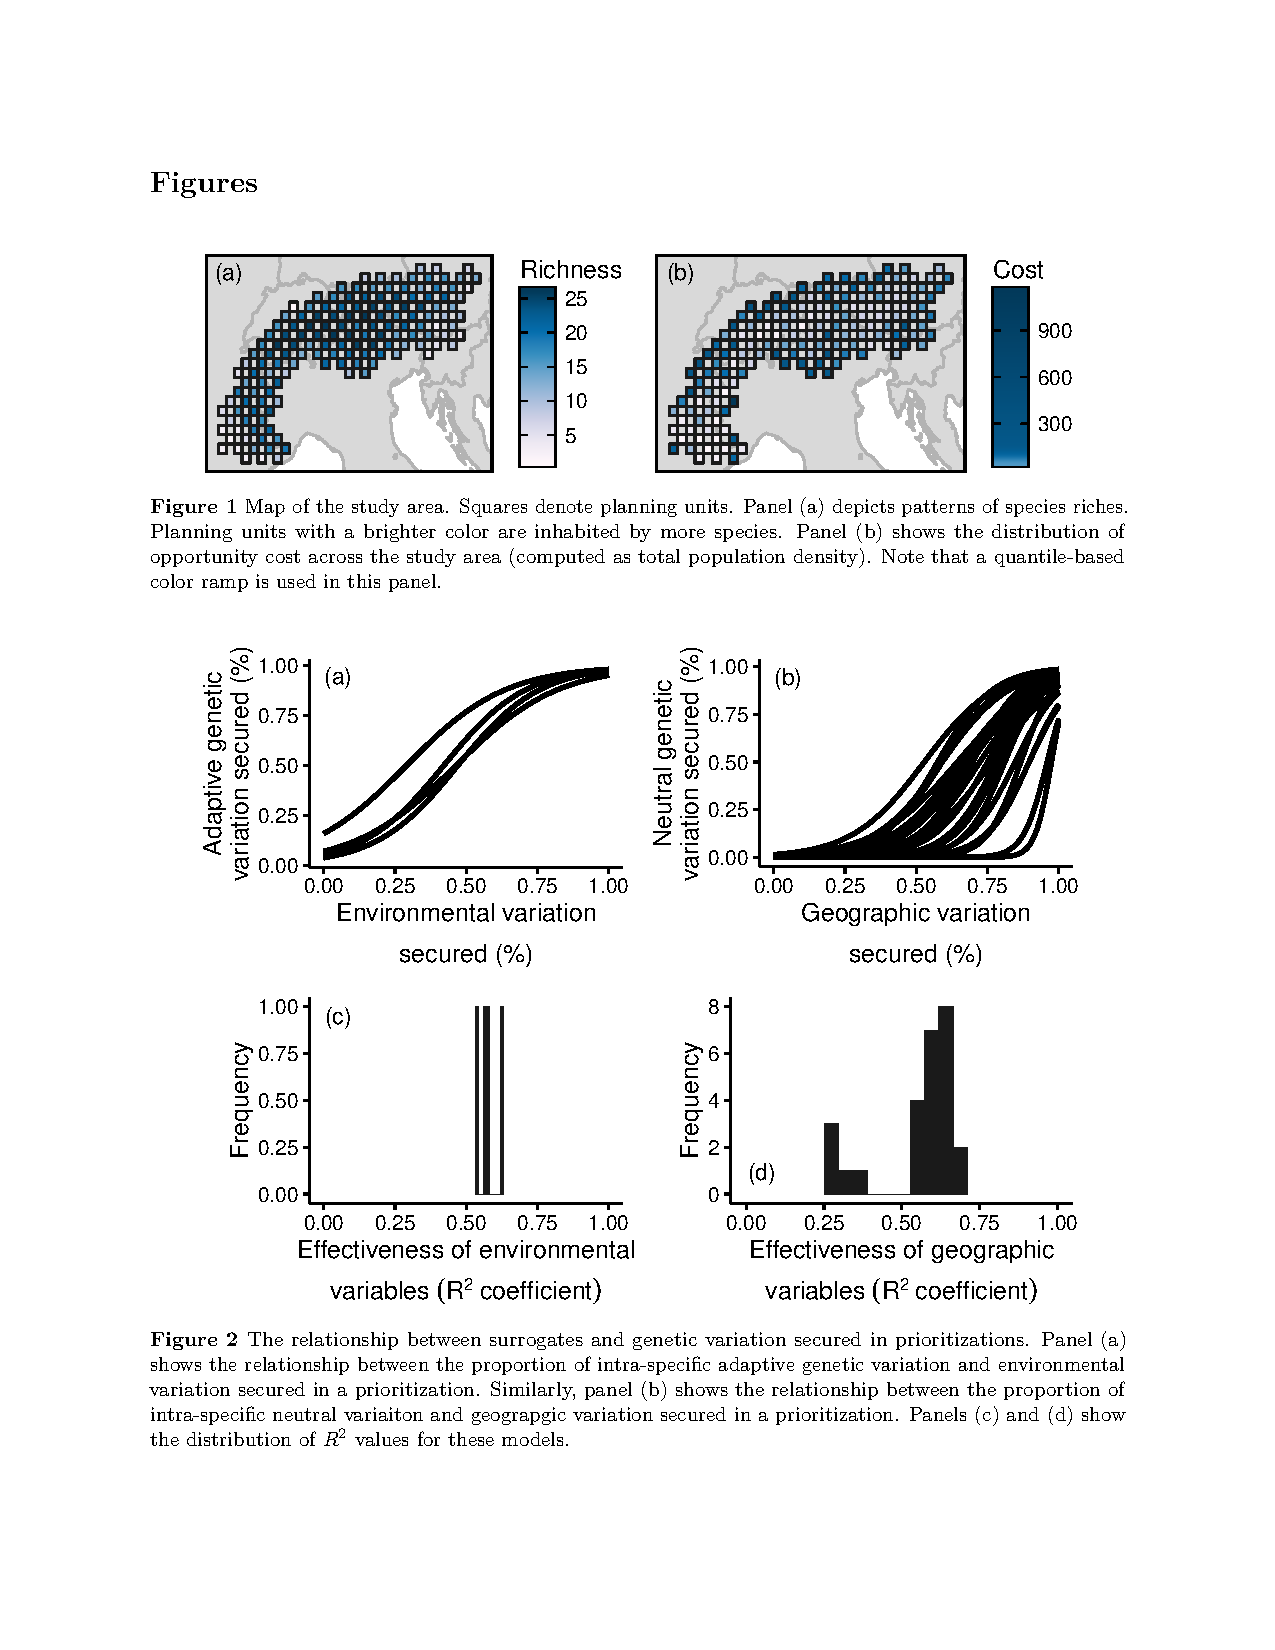
\includepdf[pages=-, pagecommand={}]{figures.pdf}
% \includepdf[pages=-, pagecommand={}]{supporting_information.pdf}

\end{document}
